\section[Problema 2]{Problema 2}

Nesse problema tivemos uma situação um pouco diferente, pois podemos observar uma rápida convergência de todos os algoritmos para o mínimo global, isso pode ser notado nas figuras \ref{fig:problema-1-genetic-algorithm-funcao-objetivo-best}, \ref{fig:problema-1-hill-climbing-com-restart-funcao-objetivo-best}, \ref{fig:problema-1-hill-climbing-funcao-objetivo} e \ref{fig:problema-1-simulated-annealing-funcao-objetivo-best}. Eu acredito que isso tenha ocorrido pela distribuição dos valores iniciais para esse problema, mas também verifica-se que os valores das funções variam muito mesmo com vizinhos próximos, diferentemente do que ocorre com o problema anterior. Logo, para esse problema vamos declarar que os 4 algoritmos se destacaram e tiveram resultados muito próximos do mínimo global. \\

O algoritmo Hill-Climbing apresentou uma escalada muito abrupta já nas primeiras iterações e um pouco antes das 200 iterações encontrou alguns mínimos locais, já abaixo de 5 e que persistiram até quase o final da sua execução. \\

O algoritmo Hill-Climbing com restart teve a sua execução muito pareceida com o Hill-Climbing, diferença essa que só se vê nos detalhes e na apreciação do gráfico basado em valores atuais visto na figura \ref{fig:problema-2-hill-climbing-com-restart-funcao-objetivo-value}. \\

O algoritmo Simulated Annealing teve uma curva ainda mais acentuada, antes mesmo da iteração 100 o algoritmo já estava bem próximo dos mínimos globais, como pode ser visto na figura \ref{fig:problema-1-simulated-annealing-funcao-objetivo-best}. Mas algo que se destacou no Simulated Annealing foram os picos máximos observados próximos das iterações 400 e 600, onde o primeiro pico atingiu um valor próximo de 350 e o segundo 250, como pode ser visto na figura \ref{fig:problema-1-simulated-annealing-funcao-objetivo-value}. \\

O Algoritmo Genético apresenta grande similaridade com o Simulated Annealing no que se refere a rápida escalada, também encontrando valores próximos dos mínimos globais um pouco antes da iteração 100, como pode ser vista na figura \ref{fig:problema-2-genetic-algorithm-funcao-objetivo-best}.

\subsection{Algoritmo Hill-Climbing}

\begin{figure}[H]
\centering
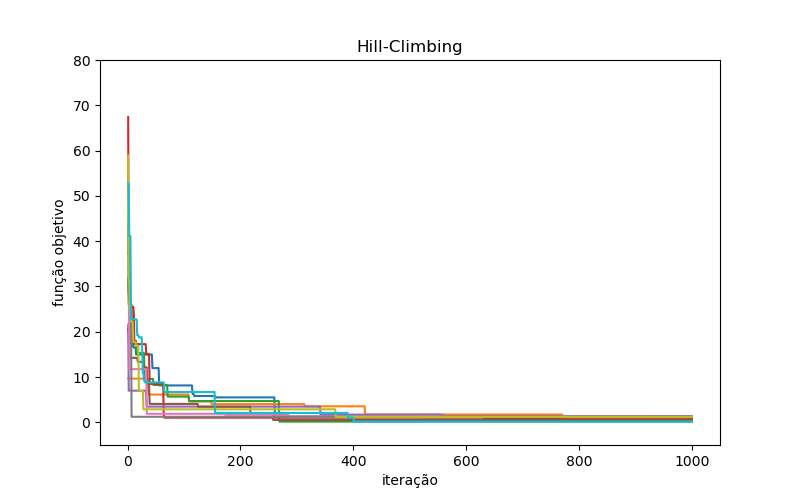
\includegraphics[width=110mm]{imagens/otima/problema-2-hill-climbing-funcao-objetivo-best.png}
\caption{Dados da execução da função objetivo durante as 10 iterações.
\label{fig:problema-2-hill-climbing-funcao-objetivo}}
\end{figure}

\subsection{Algoritmo Hill-Climbing com Restart}

\begin{figure}[H]
\centering
  \begin{minipage}[b]{0.48\textwidth}
    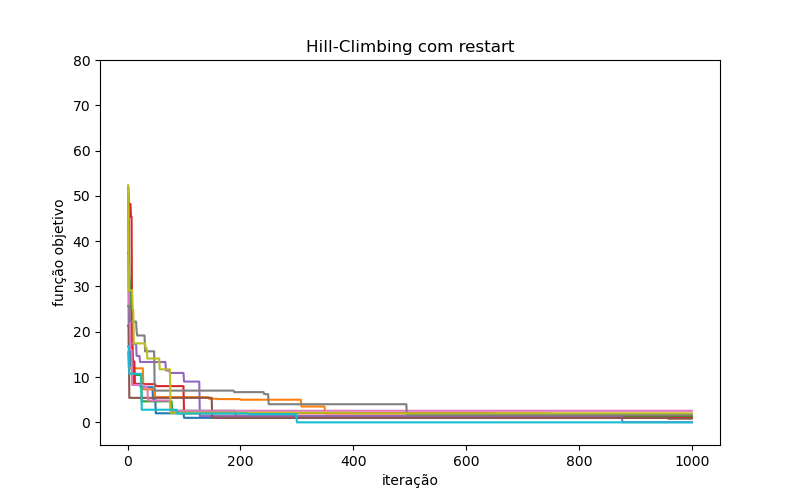
\includegraphics[width=88mm]{imagens/otima/problema-2-hill-climbing-com-restart-funcao-objetivo-best.png}
    \caption{Dados da execução da função objetivo durante as 10 iterações por melhor valor.
    \label{fig:problema-2-hill-climbing-com-restart-funcao-objetivo-best}}
  \end{minipage}
  \hfill
  \begin{minipage}[b]{0.48\textwidth}
    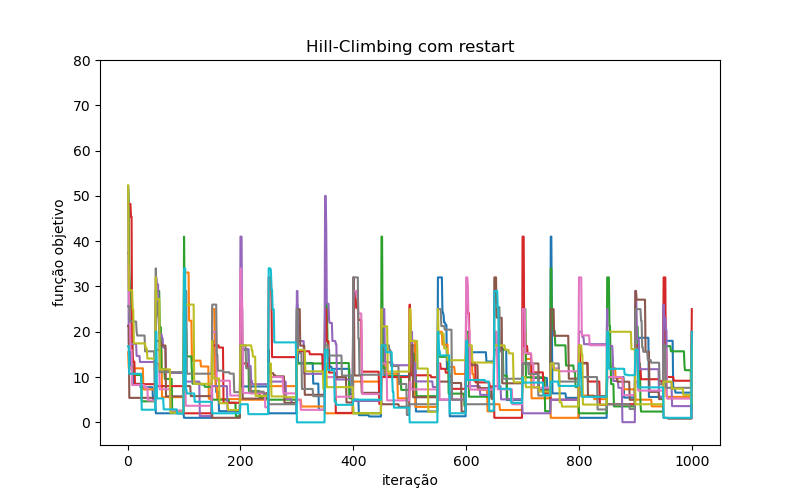
\includegraphics[width=88mm]{imagens/otima/problema-2-hill-climbing-com-restart-funcao-objetivo-value.png}
    \caption{Dados da execução da função objetivo durante as 10 iterações por valor atual.
    \label{fig:problema-2-hill-climbing-com-restart-funcao-objetivo-value}}
  \end{minipage}
\end{figure}

\subsection{Simulated Annealing}

\begin{figure}[H]
\centering
  \begin{minipage}[b]{0.48\textwidth}
    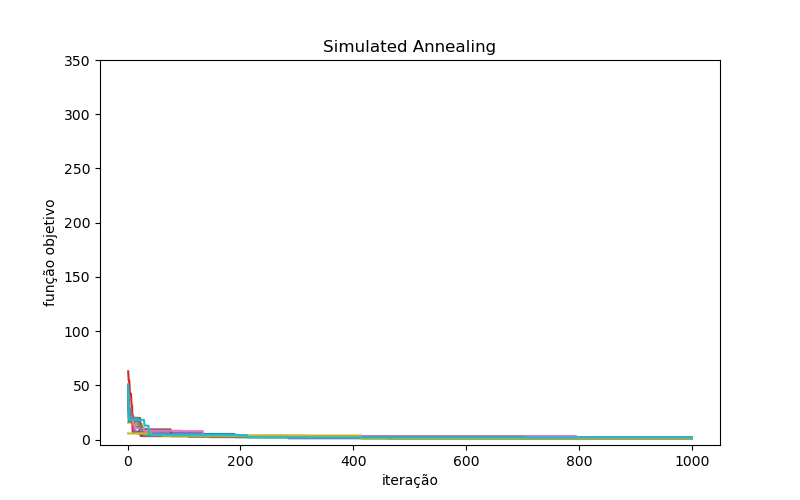
\includegraphics[width=88mm]{imagens/otima/problema-2-simulated-annealing-funcao-objetivo-best.png}
    \caption{Dados da execução da função objetivo durante as 10 iterações por melhor valor.
    \label{fig:problema-2-simulated-annealing-funcao-objetivo-best}}
  \end{minipage}
  \hfill
  \begin{minipage}[b]{0.48\textwidth}
    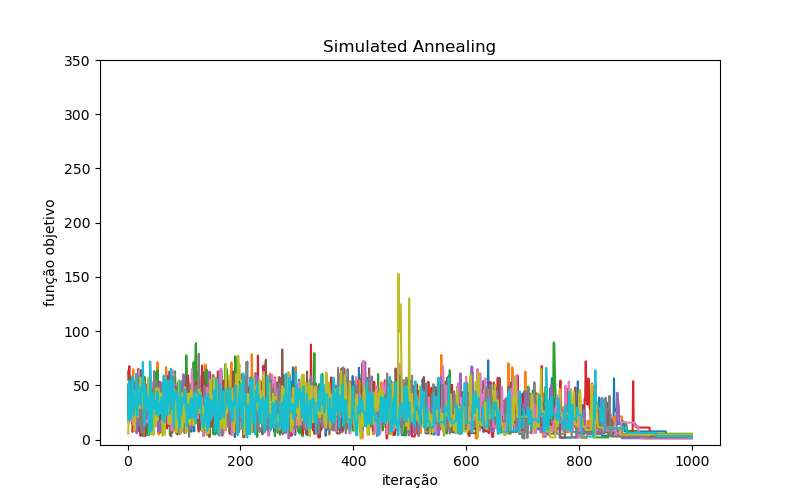
\includegraphics[width=88mm]{imagens/otima/problema-2-simulated-annealing-funcao-objetivo-value.png}
    \caption{Dados da execução da função objetivo durante as 10 iterações por valor atual.
    \label{fig:problema-2-simulated-annealing-funcao-objetivo-value}}
  \end{minipage}
\end{figure}

\subsection{Algoritmo Genético}

\begin{figure}[H]
\centering
  \begin{minipage}[b]{0.48\textwidth}
    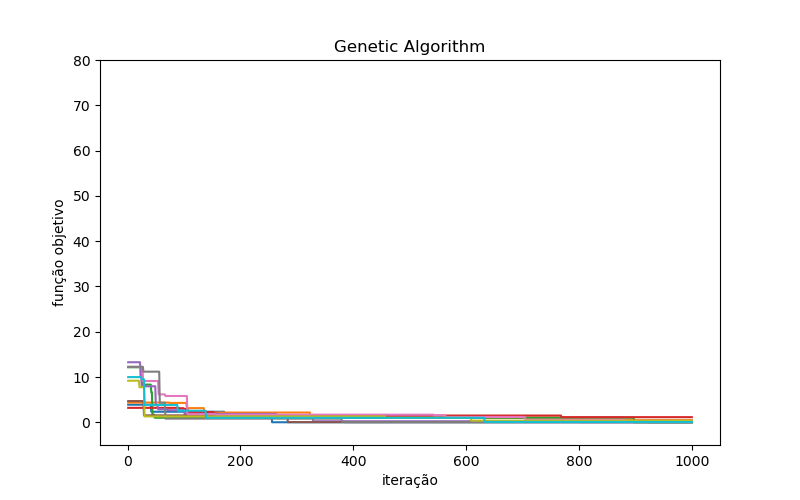
\includegraphics[width=88mm]{imagens/otima/problema-2-genetic-algorithm-funcao-objetivo-best.png}
    \caption{Dados da execução da função objetivo durante as 10 iterações por melhor valor.
    \label{fig:problema-2-genetic-algorithm-funcao-objetivo-best}}
  \end{minipage}
  \hfill
  \begin{minipage}[b]{0.48\textwidth}
    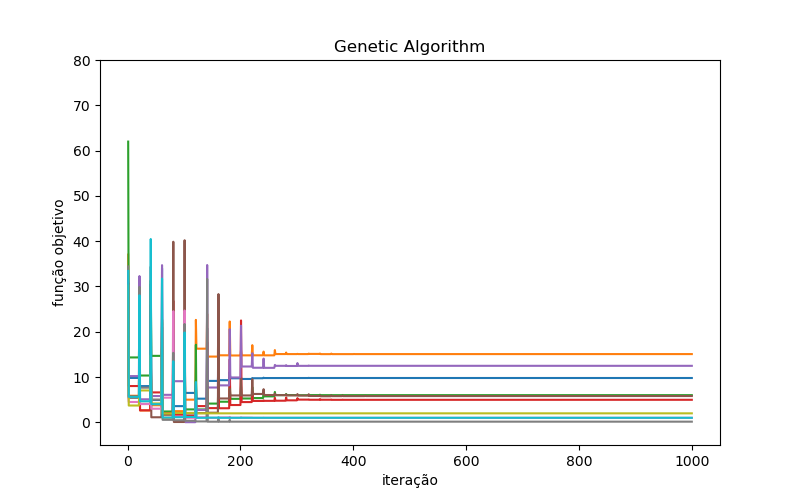
\includegraphics[width=88mm]{imagens/otima/problema-2-genetic-algorithm-funcao-objetivo-value.png}
    \caption{Dados da execução da função objetivo durante as 10 iterações por valor atual.
    \label{fig:problema-2-genetic-algorithm-funcao-objetivo-value}}
  \end{minipage}
\end{figure}